\subsection{PM2.5 Monitor data from US EPA AQS Air Data Query Tool}

\subsubsection*{Data Source}

\begin{itemize}[nolistsep]
\item \textbf{Contact}

Can email the Air Quality Analysis Group (U.S. EPA Office of Air Quality Planning and Standards) on their website at \url{https://www.epa.gov/outdoor-air-quality-data/forms/contact-us-about-outdoor-air-quality-data}


\item \textbf{Citation/Link}

United States Environmental Protection Agency. \textit{Pre-Generated Data Files: Daily Summary Files, PM2.5 FRM/FEM Mass (88101) and PM2.5 non FRM/FEM Mass (88502), 2008-2014}. \url{https://aqs.epa.gov/aqsweb/airdata/download_files.html#Daily} 
\item \textbf{Data (local)}
\item \textbf{Geographic Extent}
\item \textbf{Temporal Extent}
2008 through 2014
\item \textbf{Acknowledgment}
\end{itemize}

\subsubsection*{Brief Description}

We will download PM\textsubscript{2.5} data from both the US EPA AQS Air Data Query Tool \citep{EPAAirData2017} and the IMPROVE monitors that capture air quality information in 
more rural areas \citep{EPANPM25IMPROVE2017} for the 11-state region (Figure \ref{fig:Map11States}) including any of the following parameter codes: 88101, 88500, 88502, 81104 \citep{EPANPM25Memo2017,EPANPM25Parameters2017,EPANAllParameters2017}. %In 2014, there were approximately 1600 PM\textsubscript{2.5} monitors (Figure \ref{fig:MapLocations}). For the 7-year study period, we anticipate approximately 1.4 million monitor-days. 

\subsubsection*{Notes}

\subsubsection*{File Format}

\subsubsection*{Data Filtering and Processing}

\subsubsection*{Final Variable(s)}

\subsubsection*{Methods}

\begin{enumerate}
\item 
\item
\end{enumerate}

\subsubsection*{Quality Control}

\subsubsection*{Script Names}

\begin{enumerate}
\item 
\end{enumerate}

\subsubsection*{Data File Names}

\begin{enumerate}
\item daily\_88101\_2008.csv
\item daily\_88101\_2009.csv
\item daily\_88101\_2010.csv
\item daily\_88101\_2011.csv
\item daily\_88101\_2012.csv
\item daily\_88101\_2013.csv
\item daily\_88101\_2014.csv
\item daily\_88502\_2008.csv
\item daily\_88502\_2009.csv
\item daily\_88502\_2010.csv
\item daily\_88502\_2011.csv
\item daily\_88502\_2012.csv
\item daily\_88502\_2013.csv
\item daily\_88502\_2014.csv
\end{enumerate} 

\begin{figure}[H] % start figure float, this method seems to have fewer options for location specifier, H, t, c, and b should work
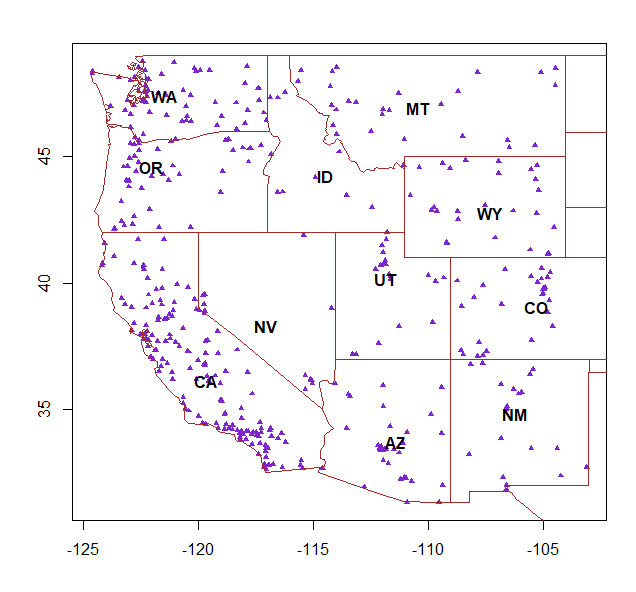
\includegraphics[width=1\textwidth]{m88101and88502notitlenorlabels.PNG} %
\caption{\label{fig:MapLocations}Map of 88101 and 88502 PM\textsubscript{2.5} Monitors.} % The text after \label{} is what shows up as the caption. Inside the brackets for \label{} is just for linking figures to text and is analogous to the AuthorYear in citations. 
\end{figure} % end figure float
